\documentclass[10pt,a4paper]{article}

% ---------- fonts and layout ----------
\usepackage[T1]{fontenc}
\usepackage[utf8]{inputenc}
\usepackage{libertinus}
\usepackage[libertine]{newtxmath}
\usepackage[final]{microtype}
\usepackage[a4paper,margin=2.0cm,top=2.2cm,bottom=2.4cm]{geometry}
\usepackage{graphicx}
\usepackage{booktabs}
\usepackage{siunitx}
\usepackage{amsmath}
\usepackage{caption}
\usepackage{subcaption}
\usepackage{enumitem}
\usepackage{xcolor}
\usepackage{tikz}
\usetikzlibrary{positioning,arrows.meta,fit,backgrounds}
\usepackage{titlesec}
\usepackage{fancyhdr}
\usepackage{needspace}
\usepackage{xurl}
\usepackage[hidelinks]{hyperref}
\usepackage[capitalise,noabbrev]{cleveref}

\graphicspath{{figures/}{../data/}}

\definecolor{ink}{HTML}{1F2937}
\definecolor{muted}{HTML}{6B7280}
\definecolor{accent}{HTML}{B45309}
\definecolor{rule}{HTML}{E5E7EB}
\definecolor{boxbg}{HTML}{F9FAFB}

\sisetup{detect-all, group-digits=integer, group-minimum-digits=4, retain-explicit-plus}
\captionsetup{font=small, labelfont={bf,color=ink}, labelsep=period, justification=justified, singlelinecheck=false}
\captionsetup[sub]{font=footnotesize, labelfont=bf, justification=centering}
\setlist{itemsep=2pt, topsep=4pt, leftmargin=1.4em}

\titleformat{\section}{\large\bfseries\color{ink}}{\thesection}{0.8em}{}
\titleformat{\subsection}{\normalsize\bfseries\color{ink}}{\thesubsection}{0.8em}{}
\titlespacing*{\section}{0pt}{1.4em}{0.5em}
\titlespacing*{\subsection}{0pt}{1.0em}{0.35em}

\pagestyle{fancy}
\fancyhf{}
\renewcommand{\headrulewidth}{0pt}
\fancyfoot[L]{\footnotesize\color{muted}Spectrally optimal light sources}
\fancyfoot[R]{\footnotesize\color{muted}\thepage}

\newcommand{\dE}{\Delta E^{*}_{ab}}
\newcommand{\dRGB}{\Delta RGB}

\hypersetup{pdftitle={Spectrally Optimal Light Sources: Designing LED Illumination to Hide or Reveal an Ishihara Numeral},
            pdfauthor={Minh Khang Tran}}

\begin{document}

% ---------- title block ----------
\thispagestyle{empty}
\begin{center}
  {\footnotesize\color{muted}\scshape Color Science Laboratory $\cdot$ University of Eastern Finland $\cdot$ COSI 2025}\\[0.9em]
  {\LARGE\bfseries\color{ink} Spectrally Optimal Light Sources}\\[0.35em]
  {\large\color{ink} Designing LED Illumination to Hide or Reveal an Ishihara Numeral}\\[0.9em]
  {\normalsize Minh Khang Tran}\\[0.2em]
  {\small\color{muted} Lab work September--October 2025 $\cdot$ report revised October 2026}
\end{center}

\vspace{0.6em}
\begin{figure}[h]
  \centering
  \begin{subfigure}{0.25\linewidth}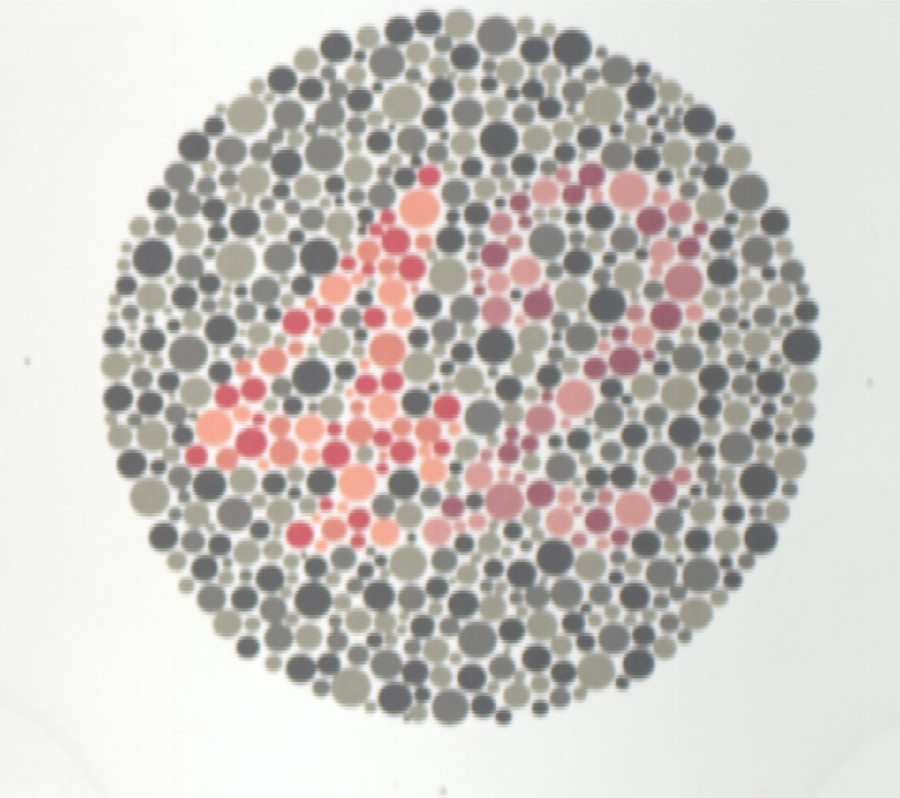
\includegraphics[width=\linewidth]{renderings/D65.jpg}\caption{D65, $\dE = 31.8$}\end{subfigure}\hfill
  \begin{subfigure}{0.25\linewidth}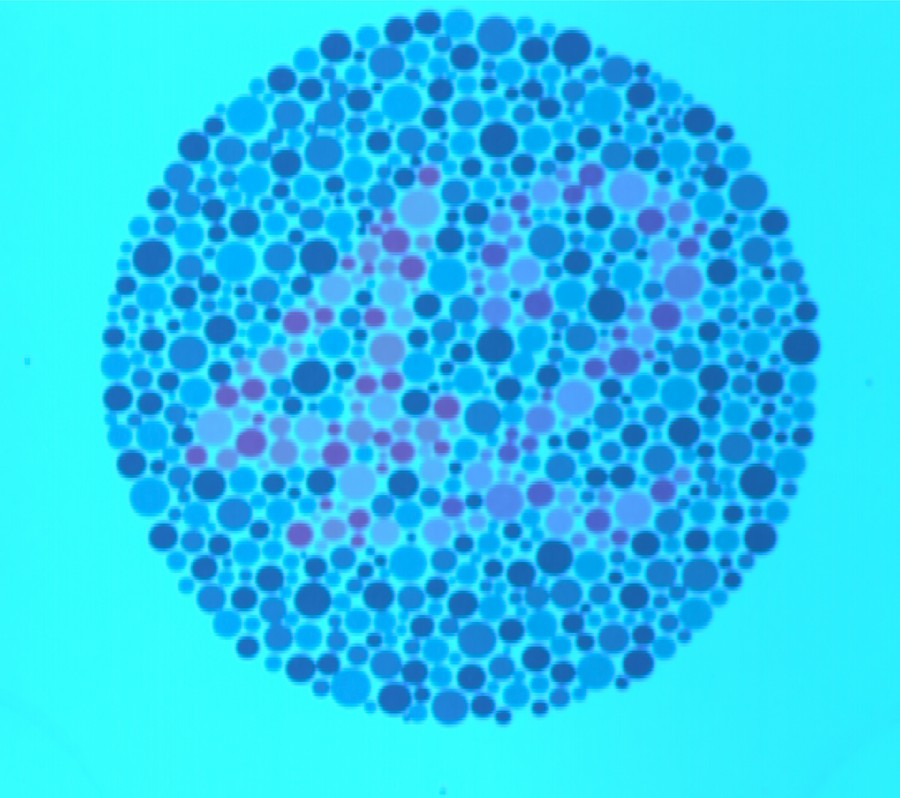
\includegraphics[width=\linewidth]{renderings/DeltaE_min.jpg}\caption{$\dE$-min light, $7.5$}\end{subfigure}\hfill
  \begin{subfigure}{0.25\linewidth}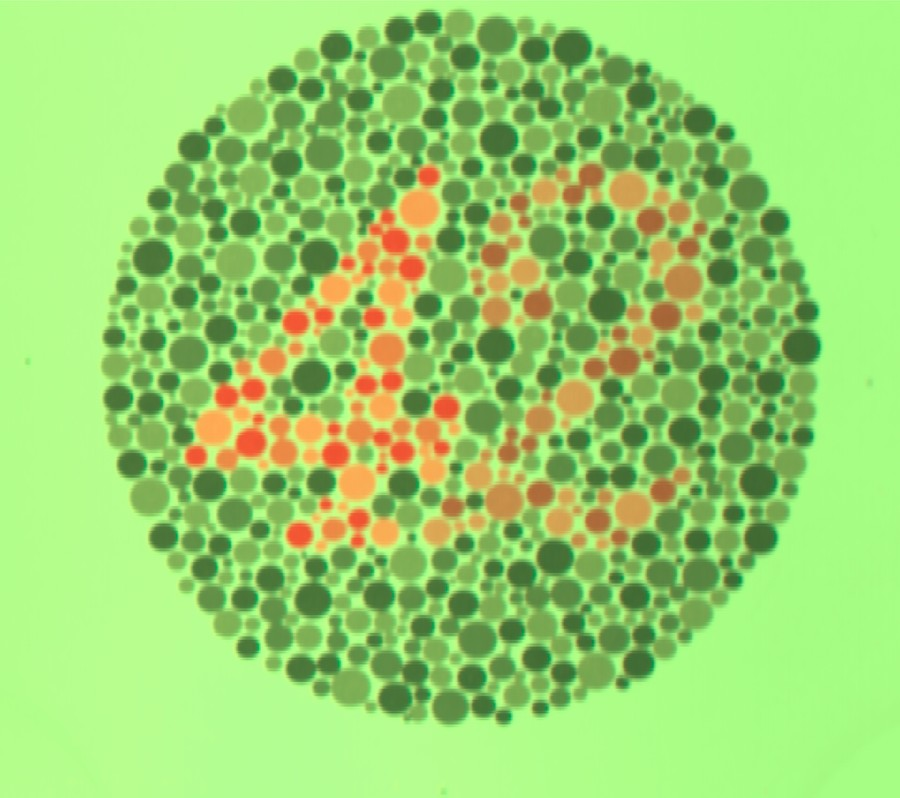
\includegraphics[width=\linewidth]{renderings/DeltaE_max.jpg}\caption{$\dE$-max light, $57.7$}\end{subfigure}
  \caption{Plate ``42'' of the Ishihara book, rendered from its measured reflectance under three illuminants. The two
  LED spectra were found by particle swarm optimisation to shrink or enlarge the colour difference between the numeral
  and the background, and were then reproduced on a tunable LED source.}
  \label{fig:teaser}
\end{figure}

\vspace{-0.4em}
\noindent\colorbox{boxbg}{\parbox{\dimexpr\linewidth-2\fboxsep}{\small
\textbf{Summary.} Two dots on an Ishihara plate, one from the numeral and one from the background, were measured
with a Specim V10E hyperspectral camera. Ten LED channels of a Ledmotive Spectra Tune Lab were measured with a
Hamamatsu PMA-12 spectrometer. Particle swarm optimisation (PSO) searched the mix of the ten channels for six
objectives: minimise or maximise CIELAB $\dE$, sRGB $\dRGB$, and Michelson luminance contrast between the two dots.
Against D65 ($\dE = 31.8$), the optimised lights reach $\dE = 7.5$ and $57.7$. Each light needs at most three of the
ten LEDs, and the $\dRGB$ and contrast objectives pick the same mix. All six lights were set on the Ledmotive, and
their emitted spectra match the predictions with Pearson $r = 0.997$--$0.999$ and \SIrange{3.5}{6.6}{\percent}
relative error. The match is in the emitted spectrum; the perceived colour difference under the real lights was not
measured.}}

% ---------- 1 ----------
\section{Question}

Colour appearance depends on the light as much as on the surface. Two surfaces whose reflectances differ only in
some wavelengths look alike under a light with little power there, and look very different under a light concentrated
there. An Ishihara plate is built on that idea: numeral and background dots are close in lightness and differ mainly in
the long wavelengths, which a red--green colour-deficient observer weighs differently.

With a light source whose spectrum can be set channel by channel, this can be turned around: \emph{which mix of the
available LEDs makes the numeral as hard, or as easy, as possible to see?} The lab answered this for one plate and three
measures of difference, and then checked that the hardware produces the spectra the optimiser asked for.

% ---------- 2 ----------
\section{Setup and data}

\begin{figure}[t]
\centering
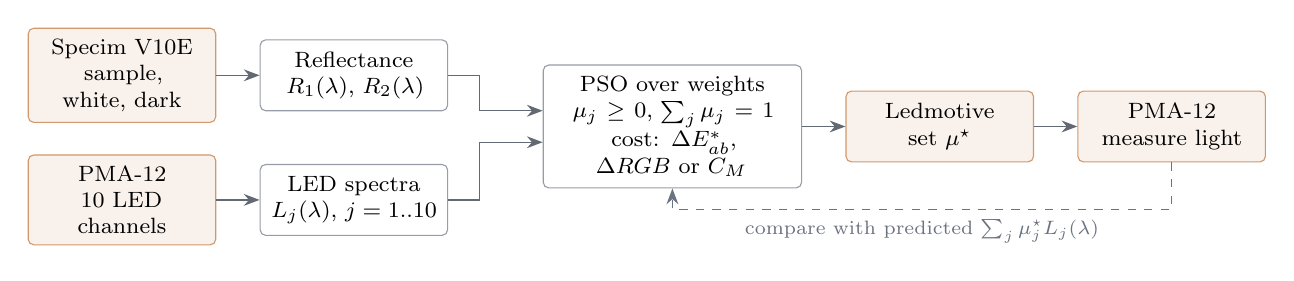
\begin{tikzpicture}[
  node distance=4mm and 5.5mm,
  box/.style={draw=muted!70, rounded corners=2pt, fill=white, align=center, font=\footnotesize, inner sep=4pt, minimum height=9mm, text width=21mm},
  hw/.style={box, fill=accent!8, draw=accent!60},
  arr/.style={-{Stealth[length=2mm]}, draw=ink!70, line width=0.5pt}]
  \node[hw]  (cam)  {Specim V10E\\ sample, white, dark};
  \node[box, right=of cam] (refl) {Reflectance\\ $R_1(\lambda)$, $R_2(\lambda)$};
  \node[hw, below=of cam] (pma)  {PMA-12\\ 10 LED channels};
  \node[box, right=of pma] (led) {LED spectra\\ $L_j(\lambda)$, $j=1..10$};
  \node[box, right=12mm of refl, yshift=-6.5mm, text width=30mm, minimum height=14mm] (pso)
        {PSO over weights $\mu_j \ge 0$, $\sum_j \mu_j = 1$\\[1pt]
         cost: $\dE$, $\dRGB$ or $C_M$};
  \node[hw, right=of pso] (src) {Ledmotive\\ set $\mu^\star$};
  \node[hw, right=of src] (chk) {PMA-12\\ measure light};
  \draw[arr] (cam) -- (refl);
  \draw[arr] (pma) -- (led);
  \draw[arr] (refl.east) -- ++(4mm,0) |- ([yshift=2mm]pso.west);
  \draw[arr] (led.east) -- ++(4mm,0) |- ([yshift=-2mm]pso.west);
  \draw[arr] (pso) -- (src);
  \draw[arr] (src) -- (chk);
  \draw[arr, dashed, draw=muted] (chk.south) -- ++(0,-6mm) -| node[pos=0.25, below, font=\scriptsize, text=muted]{compare with predicted $\sum_j \mu^\star_j L_j(\lambda)$} (pso.south);
\end{tikzpicture}
\caption{Pipeline. Orange boxes are lab instruments; white boxes are computation. Only the last comparison runs on the
real light source.}
\label{fig:pipeline}
\end{figure}

\paragraph{Plate.} Plate ``42'' of the \emph{Ishihara Color Deficiency Test} book was scanned with a Specim V10E
push-broom camera (2144 pixels per line, 586 lines, 270 bands at about \SI{2.5}{nm} from 323 to \SI{1008}{nm}).
Reflectance was computed per band as $R = (S - D)/(W - D)$ from the sample, white-reference and dark-reference scans,
and the 120 bands between 400 and \SI{700}{nm}, the range the LED source covers, were kept. One pixel was taken from a
pink dot of the numeral ($R_1$) and one from a grey dot of the background ($R_2$). \Cref{fig:reflectance} shows the two
spectra: they track each other up to about \SI{570}{nm}, after which $R_1$ rises to nearly 1 while $R_2$ stays near 0.4.

\paragraph{Light source.} The Ledmotive Spectra Tune Lab has ten channels. Each was driven alone and measured with the
PMA-12 spectrometer (\SI{85}{ms} exposure, mean of 10 spectra), then resampled to the 120 reflectance bands
(\cref{fig:leds}). The peaks lie at 430, 447, 466, 474, 504, 524, 546, 596, 637 and \SI{660}{nm}; channel 7 is a broad
phosphor-type emitter, the others are narrow.

\begin{figure}[t]
  \centering
  \begin{minipage}[t]{0.40\linewidth}
    \centering
    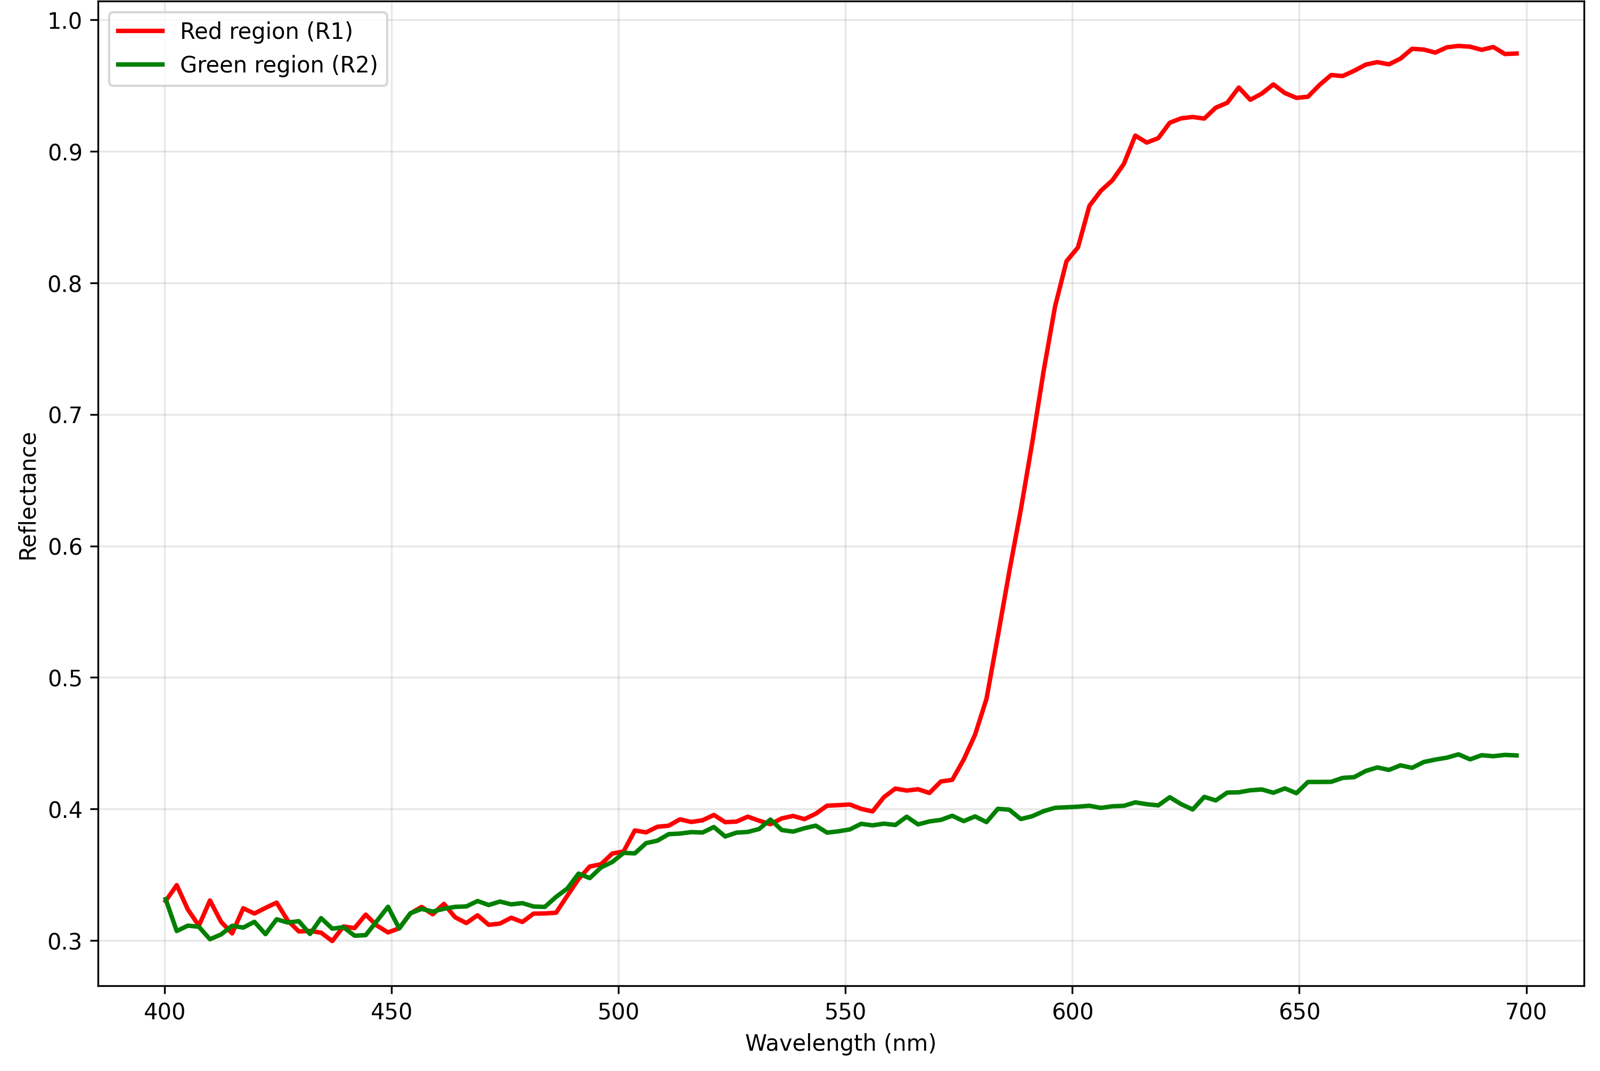
\includegraphics[width=\linewidth]{reflectance_2025.png}
    \caption{Reflectance of the numeral dot $R_1$ (red) and the background dot $R_2$, plotted by the 2025 run (the
    legend there calls $R_2$ ``green''; it is the grey background). The raw cube has since been lost, so this plot is
    the only remaining record of the two spectra.}
    \label{fig:reflectance}
  \end{minipage}\hfill
  \begin{minipage}[t]{0.56\linewidth}
    \centering
    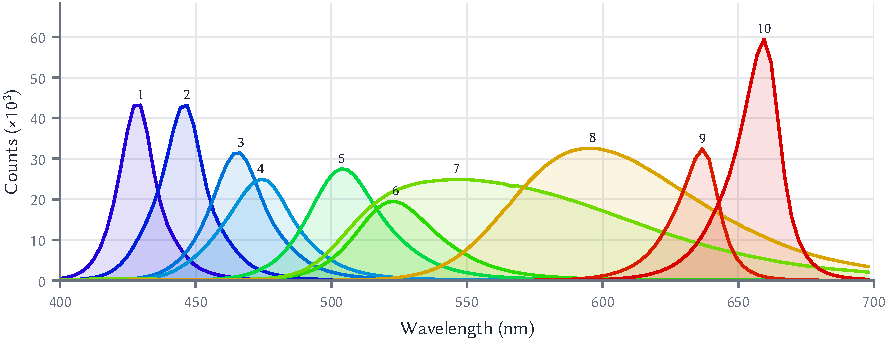
\includegraphics[width=\linewidth]{leds.pdf}
    \caption{The ten LED channels as measured by the PMA-12, in raw counts on the reflectance grid. Numbers mark the
    channel index.}
    \label{fig:leds}
  \end{minipage}
\end{figure}

% ---------- 3 ----------
\section{Method}

\paragraph{Colour of a dot under a light.} For a light $L(\lambda)$ and a reflectance $R(\lambda)$ the CIE 1931
tristimulus values are
\begin{equation}
  X = k \sum_\lambda R(\lambda)\,L(\lambda)\,\bar{x}(\lambda), \qquad
  k = \frac{100}{\sum_\lambda L(\lambda)\,\bar{y}(\lambda)},
\end{equation}
and likewise for $Y$ and $Z$, so a perfect white has $Y = 100$ under any light. Three costs follow:
\begin{itemize}
  \item $\dE$: Euclidean distance in CIELAB, with the D65 white point for every light (\cref{sec:limits}).
  \item $\dRGB$: Euclidean distance between gamma-encoded sRGB values in $[0,1]$.
  \item Michelson contrast $C_M = |g_1 - g_2|/(g_1 + g_2)$, with grey level $g = 0.2125R + 0.7154G + 0.0721B$.
\end{itemize}
A light that pushes either dot outside the sRGB gamut is treated as infeasible, which keeps the optimiser to colours a
display could show.

\paragraph{Search space.} A candidate light is a convex mix of the ten channels,
\begin{equation}
  L_\mu(\lambda) = \sum_{j=1}^{10} \mu_j L_j(\lambda), \qquad \mu_j \ge 0, \quad \sum_j \mu_j = 1 .
\end{equation}
Only the relative mix matters, because $k$ removes the overall level.

\paragraph{Optimiser.} PSO moves a swarm of candidate weight vectors, each pulled towards its own best position and the
swarm's best. After every step the weights are clipped at zero and rescaled to sum to one. The run used 200 particles,
200 iterations, inertia $c_0 = 0.95$ and attraction weights $c_1 = c_2 = 5$, once per objective (six runs).

% ---------- 4 ----------
\section{Results}

\subsection{The optimised lights}

\begin{table}[t]
  \centering
  \caption{Cost under D65 and under the optimised light. Change is relative to D65.}
  \label{tab:results}
  \small
  \begin{tabular}{l S[table-format=2.4] S[table-format=2.4] S[table-format=+3.1] S[table-format=2.4] S[table-format=+3.1]}
    \toprule
     & {D65} & {Minimised} & {Change (\%)} & {Maximised} & {Change (\%)} \\
    \midrule
    $\dE$          & 31.8197 & 7.5120 & -76.4 & 57.7057 & +81.4 \\
    $\dRGB$        & 0.2991  & 0.1988 & -33.5 & 0.7450  & +149.1 \\
    Contrast $C_M$ & 0.0494  & 0.0398 & -19.4 & 0.1124  & +127.6 \\
    \bottomrule
  \end{tabular}
\end{table}

\begin{figure}[t]
  \centering
  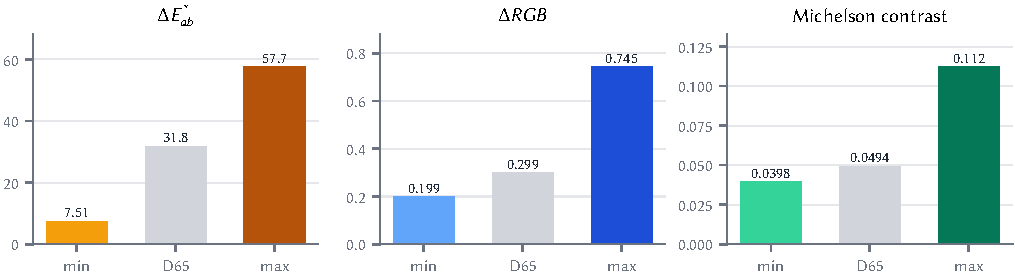
\includegraphics[width=0.92\linewidth]{metrics.pdf}
  \caption{The same numbers as \cref{tab:results}: each cost under the minimising light, D65, and the maximising light.}
  \label{fig:metrics}
\end{figure}

Every objective moved well away from D65 (\cref{tab:results,fig:metrics}). The largest relative gains are in the
maximisation direction. The minimisations are bounded by the gamut constraint and by the dots' shared reflectance below
\SI{570}{nm}: no mix of these LEDs makes the two dots identical, and luminance contrast falls by only a fifth.

\begin{figure}[h]
  \centering
  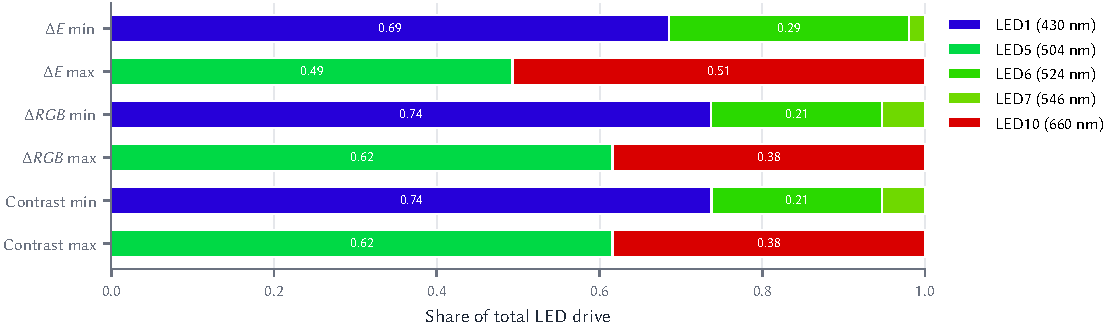
\includegraphics[width=0.98\linewidth]{weights.pdf}
  \caption{LED mix chosen for each objective. Unused channels are omitted.}
  \label{fig:weights}
\end{figure}

\Cref{fig:weights} shows how the optimiser got there.
\begin{enumerate}
  \item \textbf{Sparse solutions.} Each light uses at most three of the ten channels. Maximising lights use the
  \SI{504}{nm} cyan-green and \SI{660}{nm} deep-red channels; minimising lights use \SI{430}{nm} violet plus the
  \SI{524}{nm} and \SI{546}{nm} greens.
  \item \textbf{The mechanism is the long-wavelength gap.} To reveal the numeral the light puts power above
  \SI{600}{nm}, where $R_1$ and $R_2$ differ most. To hide it the light removes that power and lights the plate where
  the two reflectances coincide.
  \item \textbf{$\dRGB$ and contrast agree.} Both maximising runs returned the same weights (0.616 / 0.384), and the
  minimising runs differ by less than 0.001 per channel. $\dE$ prefers a more even cyan/red split (0.49 / 0.51) when
  maximising.
\end{enumerate}

\begin{figure}[t]
  \centering
  \setlength{\tabcolsep}{2pt}
  \begin{tabular}{cccc}
    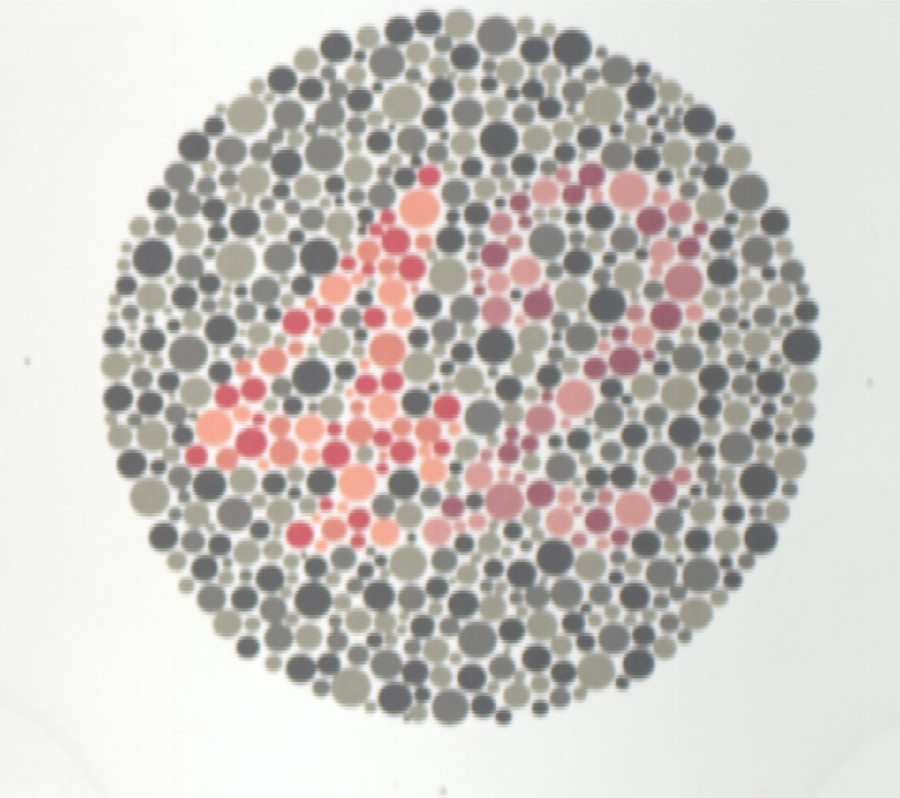
\includegraphics[width=0.235\linewidth]{renderings/D65.jpg} &
    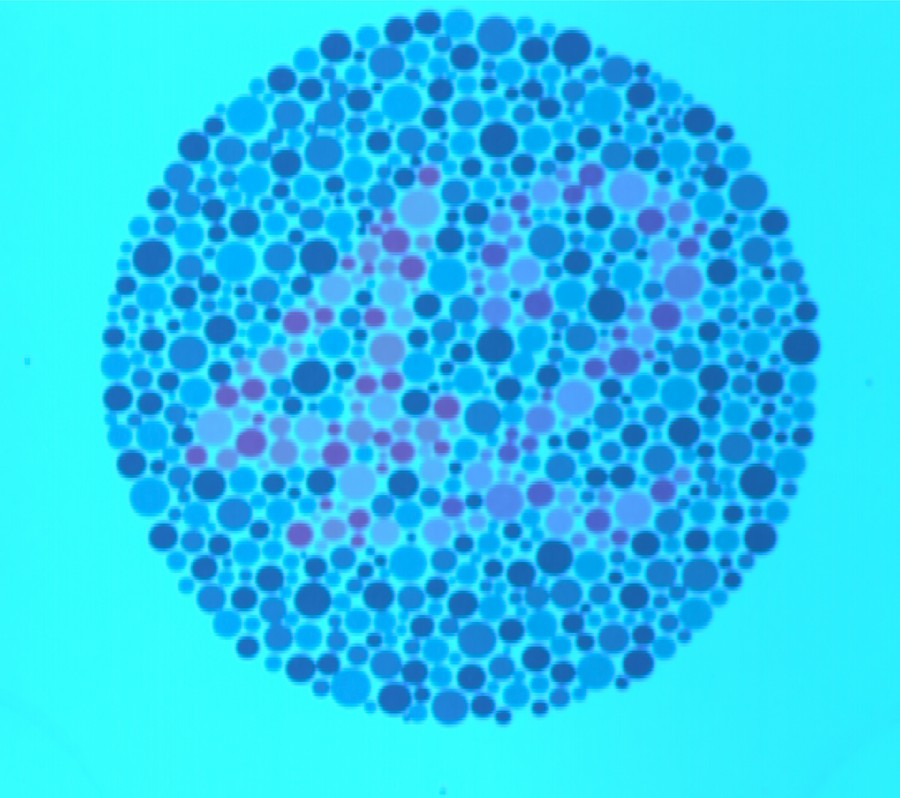
\includegraphics[width=0.235\linewidth]{renderings/DeltaE_min.jpg} &
    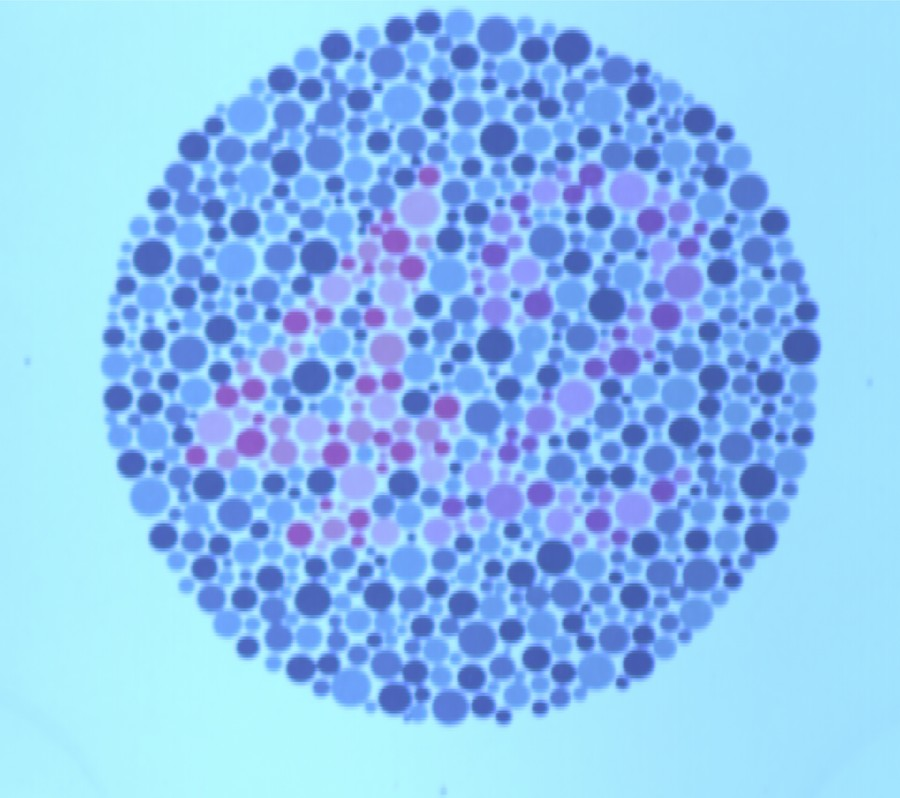
\includegraphics[width=0.235\linewidth]{renderings/DeltaRGB_min.jpg} &
    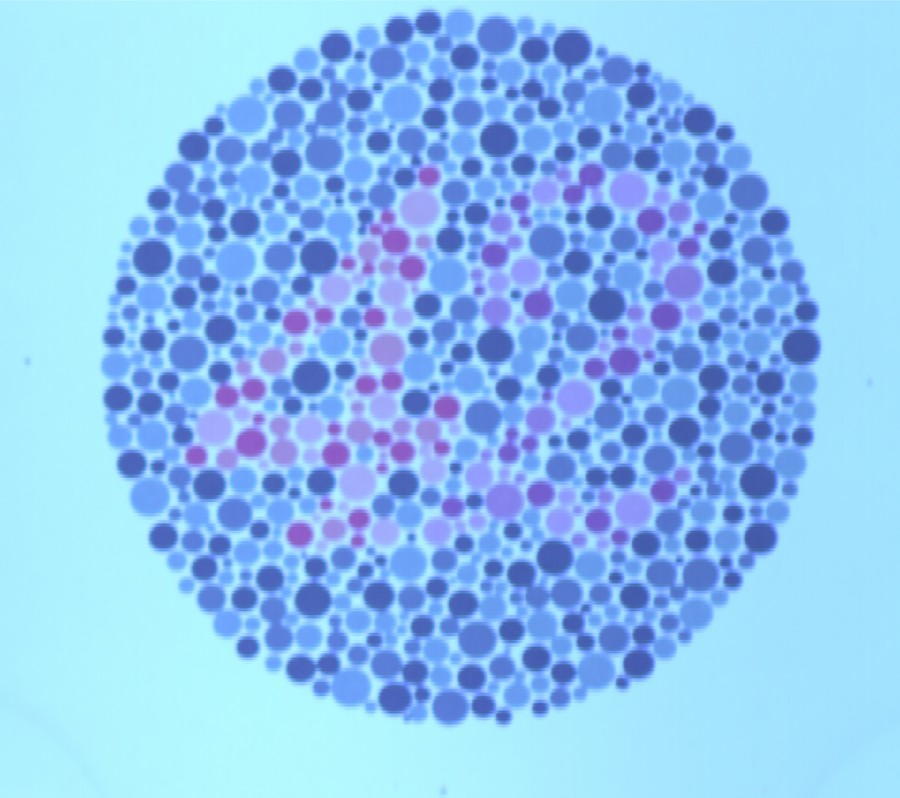
\includegraphics[width=0.235\linewidth]{renderings/Contrast_min.jpg} \\[-1pt]
    \footnotesize D65 & \footnotesize $\dE$ min & \footnotesize $\dRGB$ min & \footnotesize Contrast min \\[3pt]
     &
    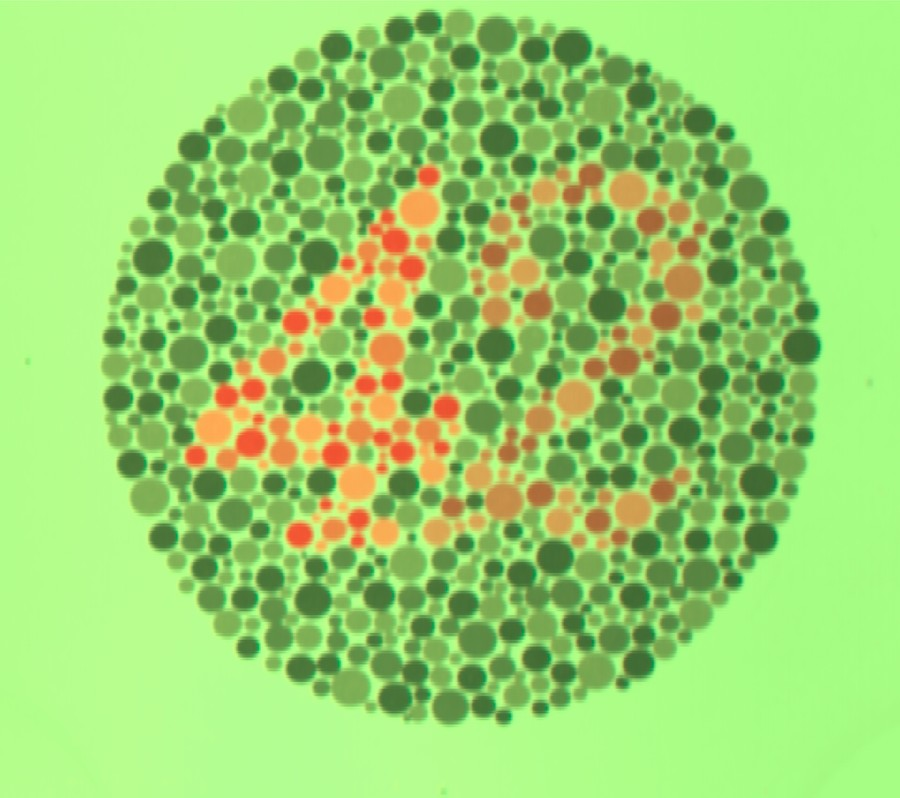
\includegraphics[width=0.235\linewidth]{renderings/DeltaE_max.jpg} &
    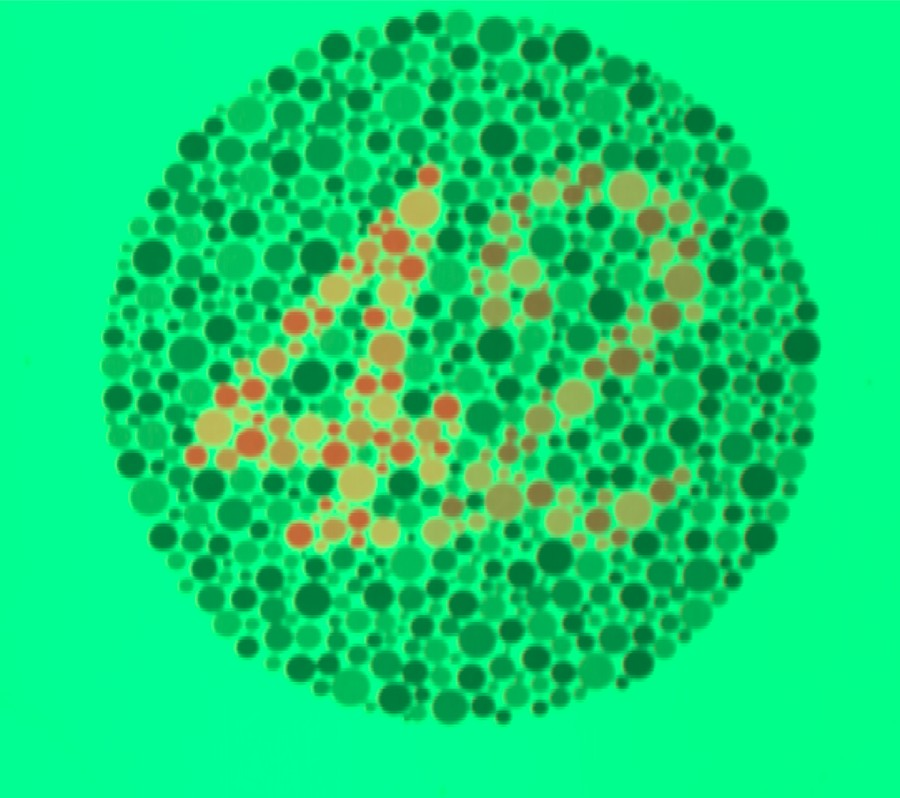
\includegraphics[width=0.235\linewidth]{renderings/DeltaRGB_max.jpg} &
    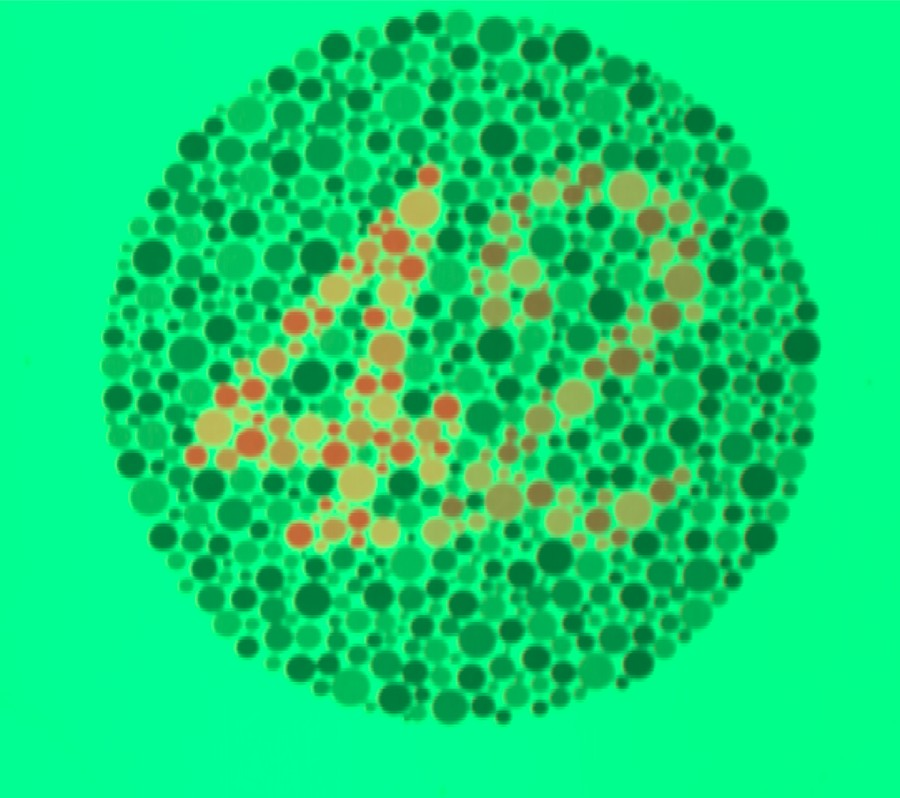
\includegraphics[width=0.235\linewidth]{renderings/Contrast_max.jpg} \\[-1pt]
     & \footnotesize $\dE$ max & \footnotesize $\dRGB$ max & \footnotesize Contrast max \\
  \end{tabular}
  \caption{The plate rendered from its reflectance cube under each light (sRGB, no white balance). Under the minimising
  lights the ``42'' nearly disappears into the background; under the maximising lights it stands out in orange.}
  \label{fig:renderings}
\end{figure}

\Cref{fig:renderings} renders the whole plate under each light. The renderings are not white-balanced, so the
background takes the colour of the light; what matters is the numeral against its surround.

\subsection{Reproduction on the LED source}

Each set of weights was entered into the Ledmotive and the emitted light measured with the PMA-12. The measured
spectrum was resampled to the 120-band grid and scaled by least squares onto the prediction, since the two
measurements were taken at different levels. \Cref{fig:validation} and \cref{tab:validation} compare them.

\begin{figure}[h]
  \centering
  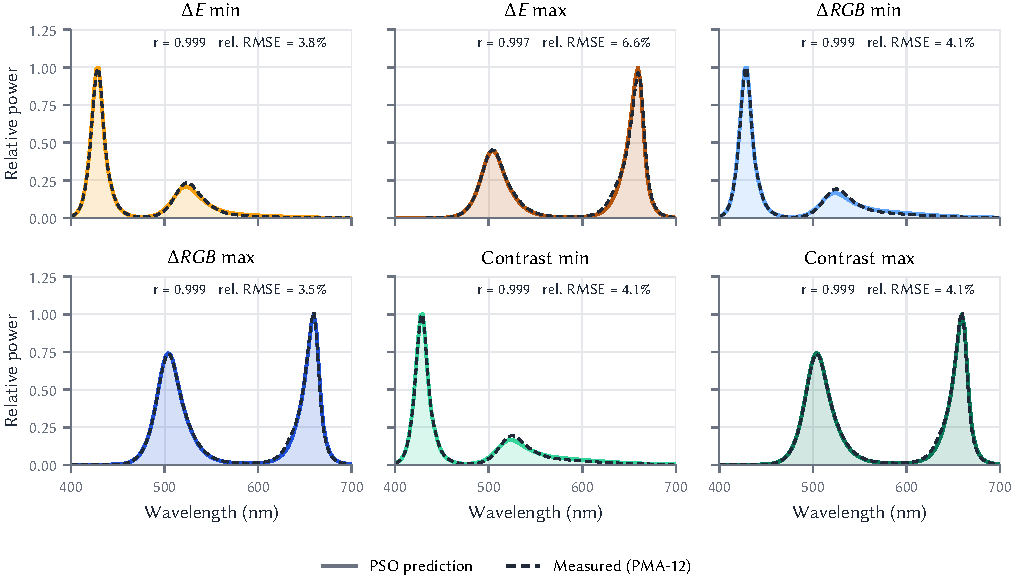
\includegraphics[width=\linewidth]{validation.pdf}
  \caption{Predicted emission $\sum_j \mu^\star_j L_j(\lambda)$ (filled) against the light the Ledmotive produced
  (dashed), each normalised to the predicted peak.}
  \label{fig:validation}
\end{figure}

\begin{table}[h]
  \centering
  \caption{Agreement between predicted and measured emission. Relative RMSE is $\lVert p - s\,m\rVert / \lVert p
  \rVert$ with $s$ the least-squares scale. Peak wavelengths agree exactly in all six cases.}
  \label{tab:validation}
  \small
  \begin{tabular}{l S[table-format=1.3] S[table-format=1.1] S[table-format=3.1]}
    \toprule
    Light & {Pearson $r$} & {Rel.\ RMSE (\%)} & {Peak (nm)} \\
    \midrule
    $\dE$ min      & 0.999 & 3.8 & 429.6 \\
    $\dE$ max      & 0.997 & 6.6 & 659.5 \\
    $\dRGB$ min    & 0.999 & 4.1 & 429.6 \\
    $\dRGB$ max    & 0.999 & 3.5 & 659.5 \\
    Contrast min   & 0.999 & 4.1 & 429.6 \\
    Contrast max   & 0.999 & 4.1 & 659.5 \\
    \bottomrule
  \end{tabular}
\end{table}

The shapes match closely. The residual is systematic: the measured secondary peak (\SI{520}{nm} for the minimising
lights, \SI{660}{nm} for $\dE$ max) comes out slightly stronger than predicted. A likely cause is that channel output is
not exactly linear in the drive setting, so mixes do not add up exactly as single-channel measurements suggest.

\begin{figure}[h]
  \centering
  \begin{subfigure}{0.23\linewidth}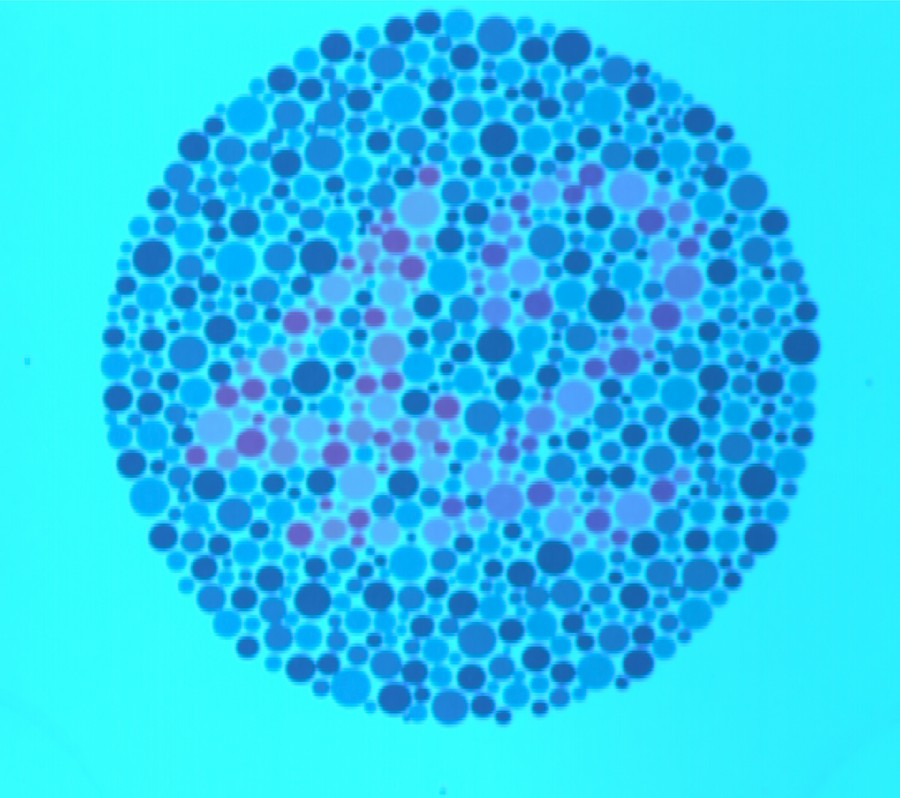
\includegraphics[width=\linewidth]{renderings/DeltaE_min.jpg}\caption{$\dE$ min, rendered}\end{subfigure}\hfill
  \begin{subfigure}{0.23\linewidth}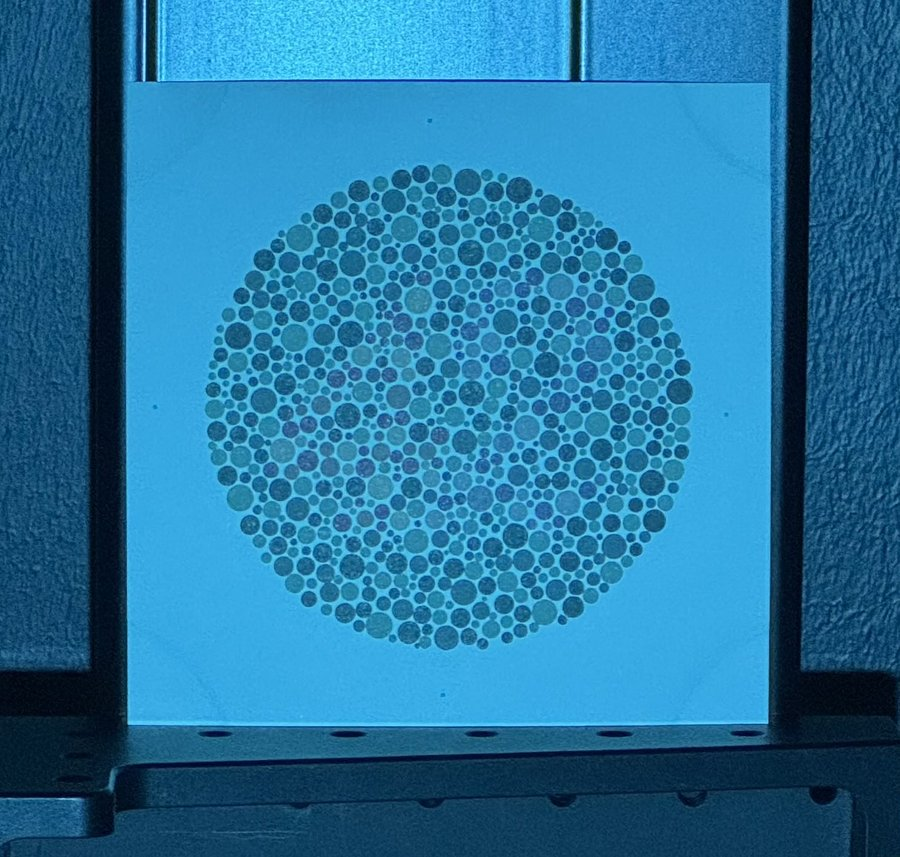
\includegraphics[width=\linewidth,height=0.92\linewidth,keepaspectratio]{photos/DeltaE_min.jpg}\caption{$\dE$ min, photo}\end{subfigure}\hfill
  \begin{subfigure}{0.23\linewidth}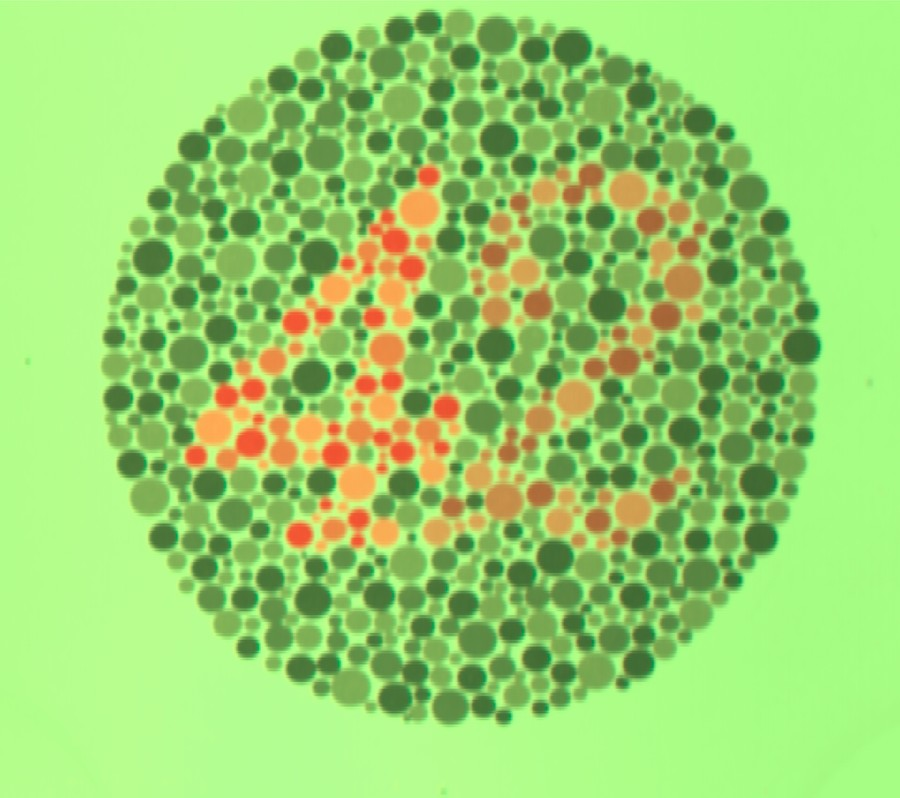
\includegraphics[width=\linewidth]{renderings/DeltaE_max.jpg}\caption{$\dE$ max, rendered}\end{subfigure}\hfill
  \begin{subfigure}{0.23\linewidth}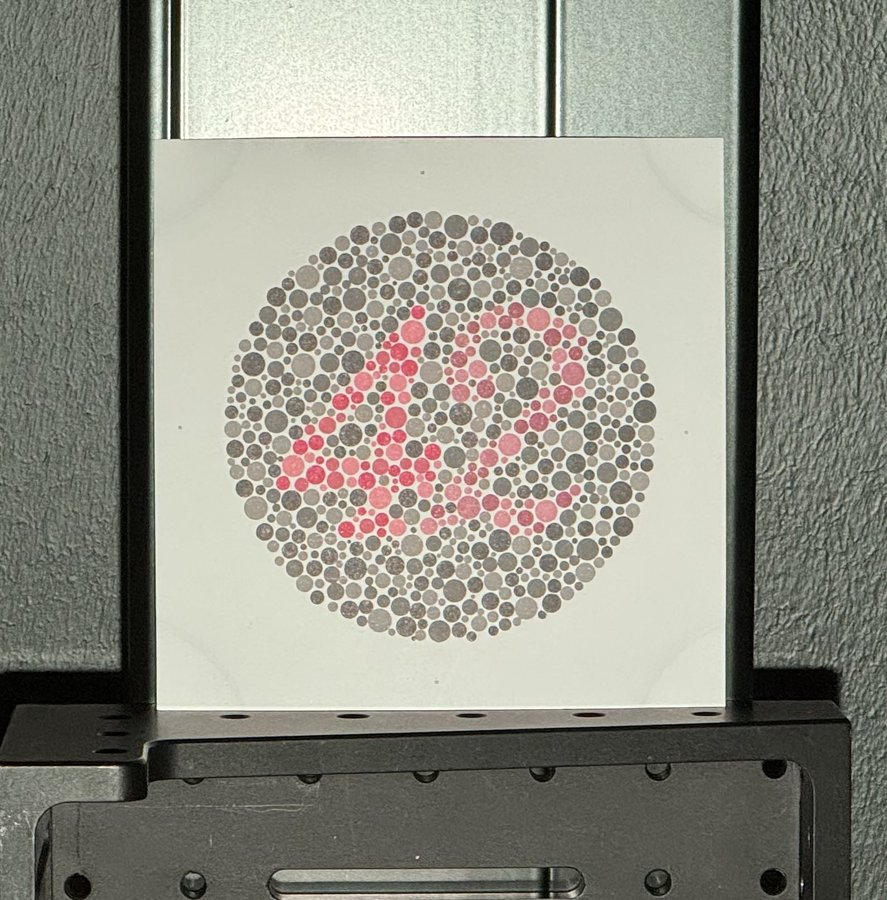
\includegraphics[width=\linewidth,height=0.92\linewidth,keepaspectratio]{photos/DeltaE_max.jpg}\caption{$\dE$ max, photo}\end{subfigure}
  \caption{Renderings next to phone photographs of the plate under the reproduced lights. The camera's automatic
  white balance neutralises the light colour, so the photos show the effect only qualitatively: the numeral fades
  under the minimising light and stands out under the maximising one.}
  \label{fig:photos}
\end{figure}

% ---------- 5 ----------
\section{Limitations}
\label{sec:limits}
\begin{itemize}
  \item \textbf{The validation covers the light, not the appearance.} It shows that the Ledmotive emits the requested
  spectra. The colour difference on the real plate under those lights was not measured (for example with a second
  hyperspectral scan or a calibrated camera), and the photos in \cref{fig:photos} are white-balanced by the phone.
  \item \textbf{No chromatic adaptation.} CIELAB uses the D65 white for every light. That describes an observer adapted
  to D65 who suddenly sees the test light; an observer adapted to the test light would see a different, probably
  smaller, $\dE$. Using the test light's own white, or a von Kries step, would be the more faithful choice.
  \item \textbf{One pixel per region.} $R_1$ and $R_2$ are single pixels, so sensor noise is part of the input (visible
  below \SI{450}{nm} in \cref{fig:reflectance}). Averaging a patch inside each dot would be more robust. The reference
  scans were also averaged over all pixels rather than per detector column.
  \item \textbf{One run per objective.} PSO is stochastic and was run once per objective with no fixed seed. Repeated
  runs would show whether the reported optima are global.
  \item \textbf{No observer test.} The plate targets colour-deficient vision, but no observer, normal or
  colour-deficient, was tested under the lights.
\end{itemize}

% ---------- 6 ----------
\section{Conclusion}

With ten measured LED channels and two measured reflectances, PSO found illuminants that cut the CIELAB difference
between an Ishihara numeral and its background from 31.8 to 7.5 or raised it to 57.7. All six lights were set on the
Ledmotive Spectra Tune Lab, and the emitted spectra matched the predictions to $r \ge 0.997$. The solutions are simple
(two or three LEDs) and easy to interpret: power above \SI{600}{nm} reveals the numeral, and removing it hides it.
The next steps would be to measure the plate under the real lights and to compute colour differences with
chromatic adaptation.

\paragraph{Code and data.} Code, LED spectra, optimised weights and the measured light spectra are available at
\url{https://github.com/tmkhang1999/Spectrally-Optimal-Light-Sources}. The comparison in
\cref{fig:validation,tab:validation} runs from those files alone; the optimisation needs the plate's reflectance cube.

\section*{References}
\small
\begin{enumerate}[label={[\arabic*]}, leftmargin=2em]
  \item J.~Kennedy and R.~Eberhart. Particle swarm optimization. \emph{Proc.\ IEEE International Conference on
  Neural Networks}, vol.~4, pp.~1942--1948, 1995.
  \item CIE 015:2018. \emph{Colorimetry}, 4th edition. Commission Internationale de l'\'Eclairage, 2018.
  \item IEC 61966-2-1:1999. \emph{Multimedia systems and equipment -- Colour measurement and management -- Part 2-1:
  Default RGB colour space -- sRGB}.
  \item Y.~Ohno. CIE fundamentals for color measurements. \emph{Proc.\ IS\&T NIP16 Conference}, pp.~540--545, 2000.
\end{enumerate}

\end{document}
